\documentclass[letterpaper,12pt]{article}

\usepackage{threeparttable}
\usepackage{geometry}
\geometry{letterpaper,tmargin=1in,bmargin=1in,lmargin=1.25in,rmargin=1.25in}
\usepackage[format=hang,font=normalsize,labelfont=bf]{caption}
\usepackage{amsmath}
\usepackage{mathrsfs}
\usepackage{multirow}
\usepackage{array}
\usepackage{delarray}
\usepackage{listings}
\usepackage{amssymb}
\usepackage{amsthm}
\usepackage{lscape}
\usepackage{natbib}
\usepackage{setspace}
\usepackage{float,color}
\usepackage[pdftex]{graphicx}
\usepackage{pdfsync}
\usepackage{verbatim}
\usepackage{placeins}
\usepackage{geometry}
\usepackage{pdflscape}
\synctex=1
\usepackage{hyperref}
\hypersetup{colorlinks,linkcolor=red,urlcolor=blue,citecolor=red}
\usepackage{bm}


\theoremstyle{definition}
\newtheorem{theorem}{Theorem}
\newtheorem{acknowledgement}[theorem]{Acknowledgement}
\newtheorem{algorithm}[theorem]{Algorithm}
\newtheorem{axiom}[theorem]{Axiom}
\newtheorem{case}[theorem]{Case}
\newtheorem{claim}[theorem]{Claim}
\newtheorem{conclusion}[theorem]{Conclusion}
\newtheorem{condition}[theorem]{Condition}
\newtheorem{conjecture}[theorem]{Conjecture}
\newtheorem{corollary}[theorem]{Corollary}
\newtheorem{criterion}[theorem]{Criterion}
\newtheorem{definition}{Definition} % Number definitions on their own
\newtheorem{derivation}{Derivation} % Number derivations on their own
\newtheorem{example}[theorem]{Example}
\newtheorem{exercise}[theorem]{Exercise}
\newtheorem{lemma}[theorem]{Lemma}
\newtheorem{notation}[theorem]{Notation}
\newtheorem{problem}[theorem]{Problem}
\newtheorem{proposition}{Proposition} % Number propositions on their own
\newtheorem{remark}[theorem]{Remark}
\newtheorem{solution}[theorem]{Solution}
\newtheorem{summary}[theorem]{Summary}
\bibliographystyle{aer}
\newcommand\ve{\varepsilon}
\renewcommand\theenumi{\roman{enumi}}
\newcommand\norm[1]{\left\lVert#1\right\rVert}

\begin{document}

\title{Math 320 Homework 5.4}
\author{Chris Rytting}
\maketitle
\subsection*{5.16}
For the first part of the piecewise function, where $n = 0$, we have the inner product given by

\begin{align*}
\langle T_0,T_0 \rangle &= \int^{1}_{-1} \frac{T_0^2}{\sqrt{1- x^2}} dx 
\\&= \int^{1}_{-1}\frac{1}{\sqrt{1- x^2}}\frac{(2^{n-1})^2}{(2^{n-1})^2} \text{cos}(0 \cdot \text{cos}^{-1}(x))dx
\\&= \int^{1}_{-1}\frac{1}{\sqrt{1- x^2}}\frac{(2^{n-1})^2}{(2^{n-1})^2} \text{cos}(0)dx
\\&= \int^{1}_{-1}\frac{1}{\sqrt{1- x^2}} 1dx
\\&= \int^{1}_{-1}\frac{1}{\sqrt{1- x^2}} dx
\\&= \pi
\end{align*}

As for the second part, where $n \neq 0$, we have the result both by integration and by remark 5.4.2.
\subsection*{5.17}

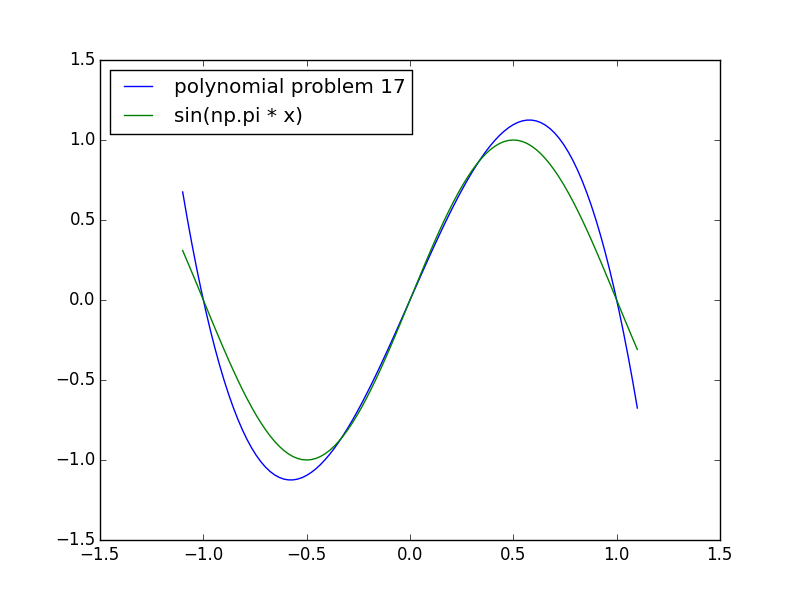
\includegraphics[scale = .75]{prob17.png}


\subsection*{5.18}

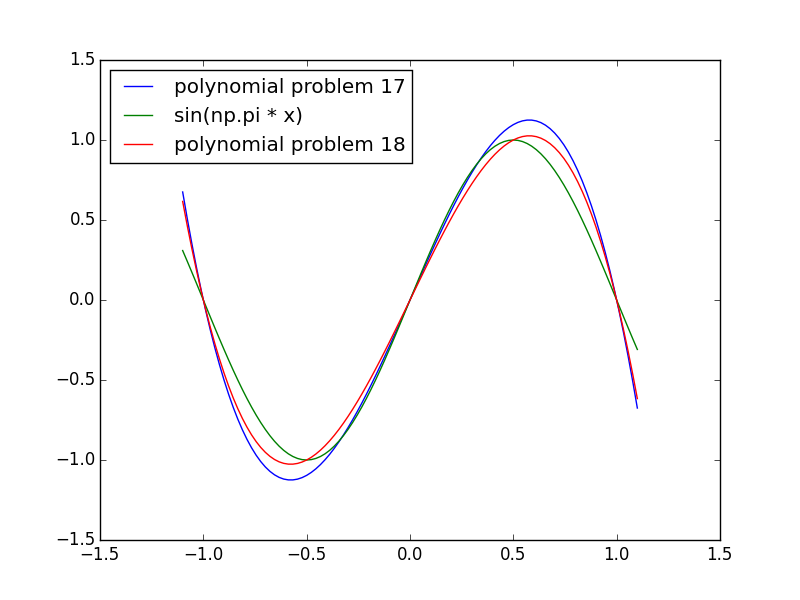
\includegraphics[scale = .75]{prob18.png}

\subsection*{5.19}
Linear change of variables function $\tilde x: [-1,1] \to [a,b] $ given by 
\[\tilde x(x) = a\left(1 - \left( \frac{x}{2} + .5\right) \right) + b\left( \frac{x}{2} + .5 \right)\]
Points of $[a,b]$ corresponding to Chebyshev roots under this map:
\[\tilde x (z_j) = a\left(1 - \left( \frac{\text{cos}(\left[\frac{\pi}{n} \left( j + \frac{1}{2} \right))\right]}{2} + .5\right) \right) + b\left( \frac{\text{cos}(\left[\frac{\pi}{n} \left( j + \frac{1}{2} \right))\right]}{2} + .5 \right) \quad j = 0,1,2,\cdots,n-1\] 
Analogue of Prop. 5.4.6:\\\\
If $|f^{(n+1)}(x)|$ is bounded by $M$ on $[a,b]$, and if $p(x)$ is the interpolating polynomial $p(x)$ of the function $f(x)$ at the Chebyshev zeros $\tilde x(z_0),x(z_1),\cdots,x(z_n)$, then 
\[ ||f - p||_{L^\infty} \leq \frac{M}{2^n(n+1)!}\]

\end{document}
